%% Poster Genetica 2026 (71o Congresso Brasileiro de Genetica)
%% Trabalho #253, Genetica de Microrganismos. Apresentacao: 01/10/2026, 17h30 a 19h30.
%% Regras do evento: 100 x 100 cm, design livre, logo do evento obrigatorio,
%% ingles ou portugues, o apresentador deve ser o primeiro autor.
%% Overleaf: Compiler = LuaLaTeX (o latexmkrc ja define isso).
%% O log informa a altura de cada coluna (procure ALTURA COLUNA); o espaco disponivel e cerca de 2242pt.

\documentclass{article}
\usepackage[paperwidth=100cm,paperheight=100cm,margin=0cm]{geometry}
\usepackage{fontspec}
\setmainfont{TeX Gyre Heros}
\usepackage{xcolor}
\usepackage{graphicx}
\usepackage{tikz}
\usepackage{enumitem}
\usepackage{ragged2e}
\graphicspath{{figures/}{logos/}}
\pagestyle{empty}
\pagecolor{white}
\setlength{\parindent}{0pt}
\setlength{\JustifyingParindent}{0pt}  % texto justificado sem recuo de paragrafo
\setlength{\parskip}{0pt}

% ---- cores: verde do logo do evento; vermelho marca este estudo nas figuras
\definecolor{evento}{HTML}{029B7C}
\definecolor{estudo}{HTML}{E31A1C}
\definecolor{texto}{HTML}{1F1F1F}
\definecolor{fundo}{HTML}{E6F4F1}

% ---- tamanhos (pt impressos)
\newcommand{\corpo}{\fontsize{24}{30}\selectfont}
\newcommand{\legenda}{\fontsize{22}{26}\selectfont}
\newcommand{\rodape}{\fontsize{19}{23}\selectfont}

% ---- nomes
\newcommand{\Hep}{\textit{Hepatozoon}}
\newcommand{\Bsaz}{\textit{Bothrops sazimai}}

% ---- grade (cm)
\newlength{\margem}\setlength{\margem}{2cm}
\newlength{\coluna}\setlength{\coluna}{47cm}
\newlength{\vao}\setlength{\vao}{2cm}
\newcommand{\topocolunas}{-15.7cm}  % inicio das colunas
\newcommand{\toporodape}{-95.3cm}   % inicio do rodape
\newcommand{\altlogo}{4.6cm}        % altura comum dos logos das afiliacoes
\newcommand{\altlogorodape}{3.4cm}  % altura comum dos logos do rodape

% ---- secoes
\newcommand{\secao}[1]{%
  \par\vspace{0.7cm}%
  {\fontsize{40}{46}\selectfont\bfseries\color{evento}#1\par}%
  \vspace{0.1cm}{\color{evento}\rule{\linewidth}{3pt}}\par\vspace{0.35cm}}
\newcommand{\subsecao}[1]{%
  \par\vspace{0.7cm}{\fontsize{30}{36}\selectfont\bfseries #1\par}\vspace{0.25cm}}

% ---- figura com legenda: #1 largura, #2 arquivo, #3 legenda
\newcommand{\figura}[3]{%
  \par\vspace{0.5cm}%
  {\centering\includegraphics[width=#1]{#2}\par}%
  \vspace{0.3cm}{\legenda\RaggedRight #3\par}}

\setlist[itemize]{leftmargin=1.1em,itemsep=0.3cm,topsep=0.1cm,parsep=0pt,
  label={\color{evento}\textbullet}}

% =====================================================================
%  COLUNA ESQUERDA
% =====================================================================
% bloco da Figura 4: medido para que o texto ao lado tenha a mesma altura
\newsavebox{\blocoquatro}
\sbox{\blocoquatro}{\begin{minipage}[t]{20.5cm}\vspace{0pt}\corpo
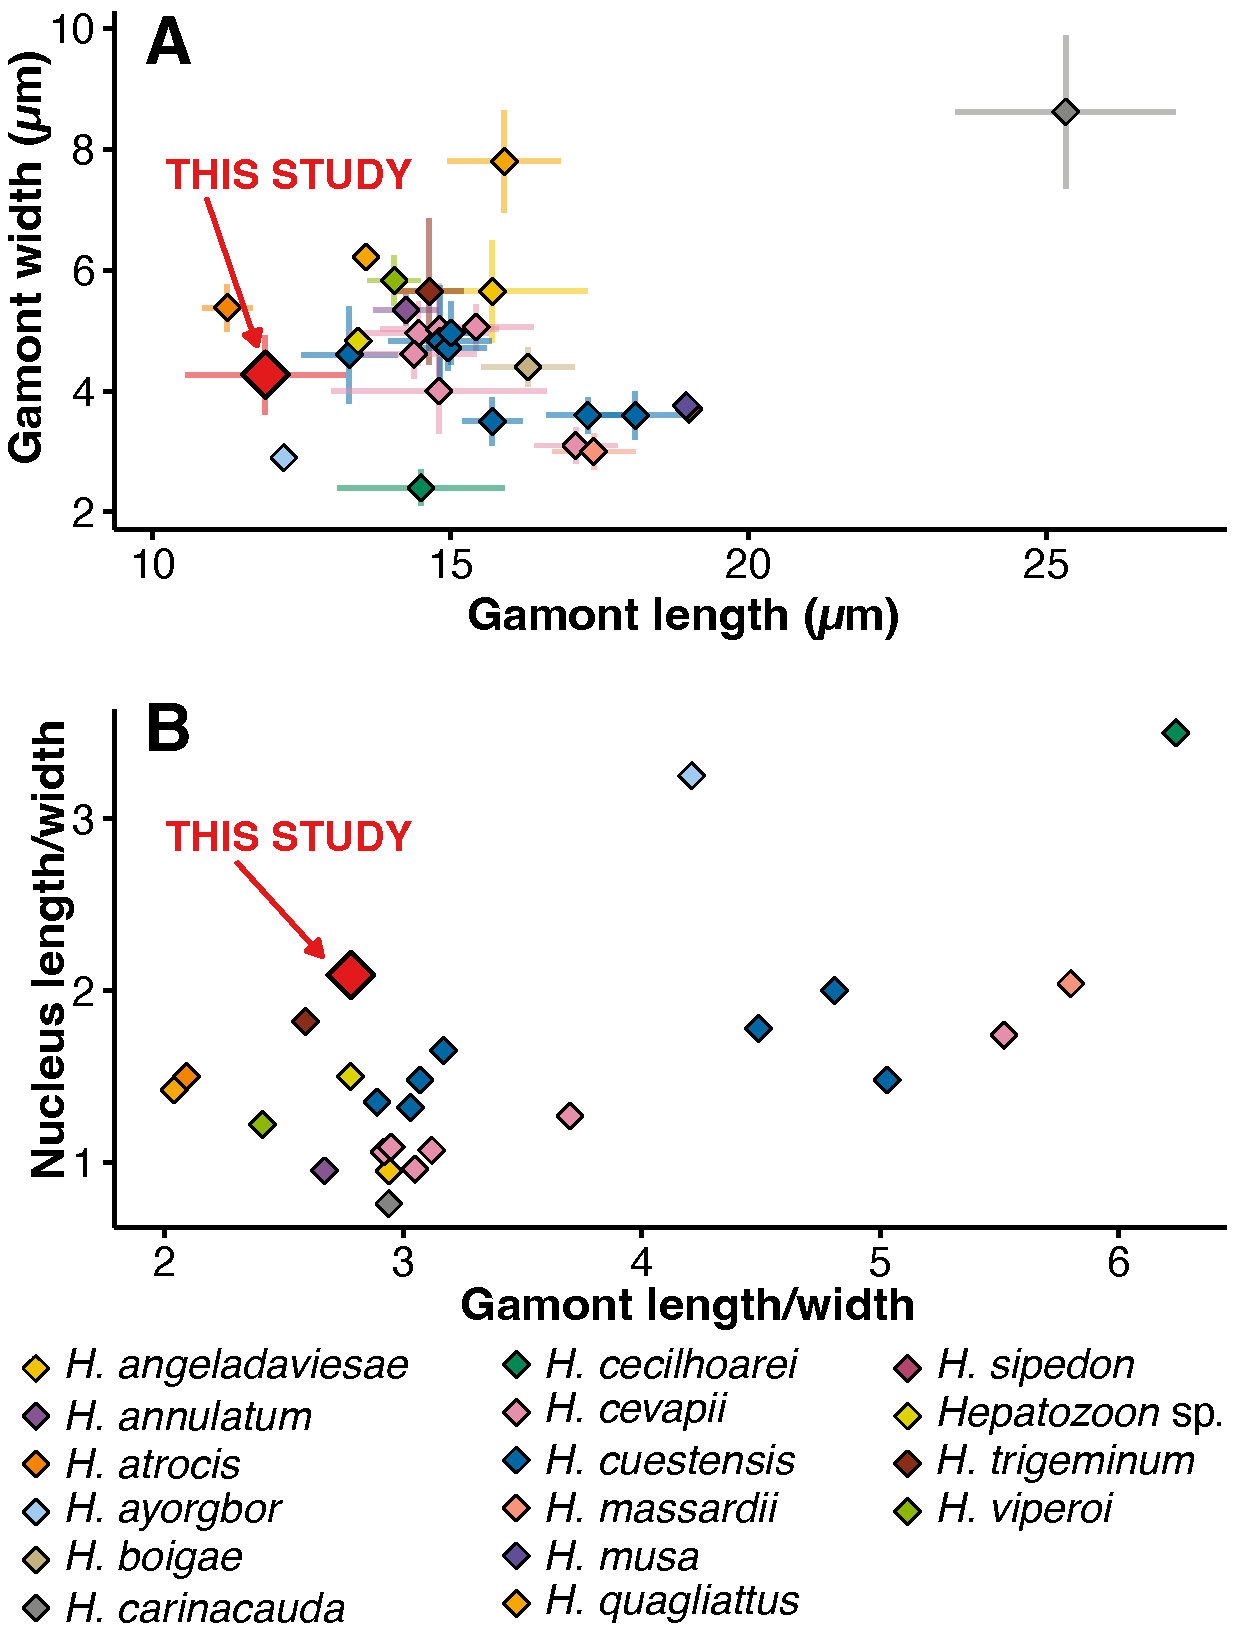
\includegraphics[width=\linewidth]{Figure_04.pdf}\par\vspace{0.3cm}
{\legenda\RaggedRight \textbf{Figure 4.} Gamonts of snake \Hep{}. A: size (mean ± SD). B: gamont and nucleus shape.\par}
\end{minipage}}
\newlength{\altquatro}
\setlength{\altquatro}{\dimexpr\ht\blocoquatro+\dp\blocoquatro\relax}

\newsavebox{\colesq}
\sbox{\colesq}{\begin{minipage}[t]{\coluna}\corpo\justifying\color{texto}
\vspace{-0.9cm}
\secao{Introduction}
\begin{minipage}[t]{30cm}\vspace{0pt}\justifying
\Hep{} (Apicomplexa: Adeleorina: Hepatozoidae) is the blood parasite most often reported in snakes. Most species were described from gamont shape and short 18S rRNA fragments. Recent studies in South America keep finding lineages that morphology alone cannot separate.

\vspace{0.4cm}
\Bsaz{} lives only on Ilha dos Franceses, Espírito Santo, Brazil (Fig.~1). Rising sea levels cut the island off from the mainland within the last 11,000 to 55,000 years\textsuperscript{2}. Its describers proposed it as Critically Endangered\textsuperscript{1}. Instituto Butantan keeps a captive colony for conservation, and health screening of these snakes also reveals their parasites.

\vspace{0.6cm}
\colorbox{fundo}{\begin{minipage}{\dimexpr\linewidth-2\fboxsep\relax}\justifying
\vspace{0.3cm}{\bfseries\color{evento}Objective.} Characterize a \Hep{} lineage found in \Bsaz{} by gamont morphology, 18S rRNA, and complete mitochondrial and apicoplast genomes, and compare it with known species.\vspace{0.3cm}
\end{minipage}}
\end{minipage}\hfill
\begin{minipage}[t]{16cm}\vspace{0pt}
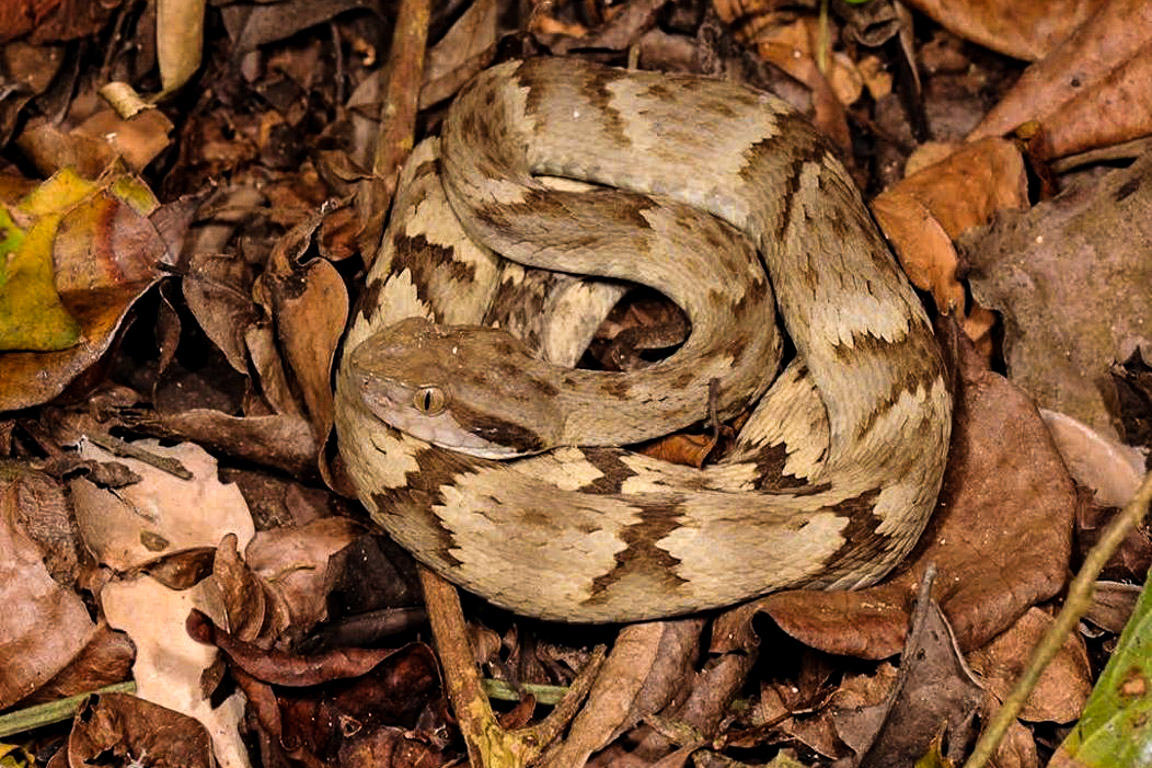
\includegraphics[width=\linewidth]{Figure_01.jpg}\par\vspace{0.3cm}
{\legenda\RaggedRight \textbf{Figure 1.} \Bsaz{} from Ilha dos Franceses. Photo: Ricardo Sawaya.\par}
\end{minipage}

\secao{Methods}
We drew blood from an adult female \Bsaz{} of the Instituto Butantan colony and compared its gamonts with 28 records of snake \Hep{} from 14 studies. We pulled parasite reads out of the host's Oxford Nanopore genome assembly (Fig.~2) and placed the 18S variants in a maximum likelihood tree of 150 adeleorin sequences.
\figura{44cm}{Figura_02.pdf}{\textbf{Figure 2.} Workflow: gamont morphometry (top) and parasite genomics (bottom). Created in BioRender (BioRender.com).}

\secao{Results}
\begin{minipage}[t][\altquatro][s]{25cm}\vspace{0pt}\justifying
{\fontsize{30}{36}\selectfont\bfseries Short gamonts with a long, narrow nucleus\par}\vspace{0.25cm}
Gamonts measured 11.9\,±\,1.3\,µm by 4.3\,±\,0.7\,µm (Fig.~3).
\vfill
{\centering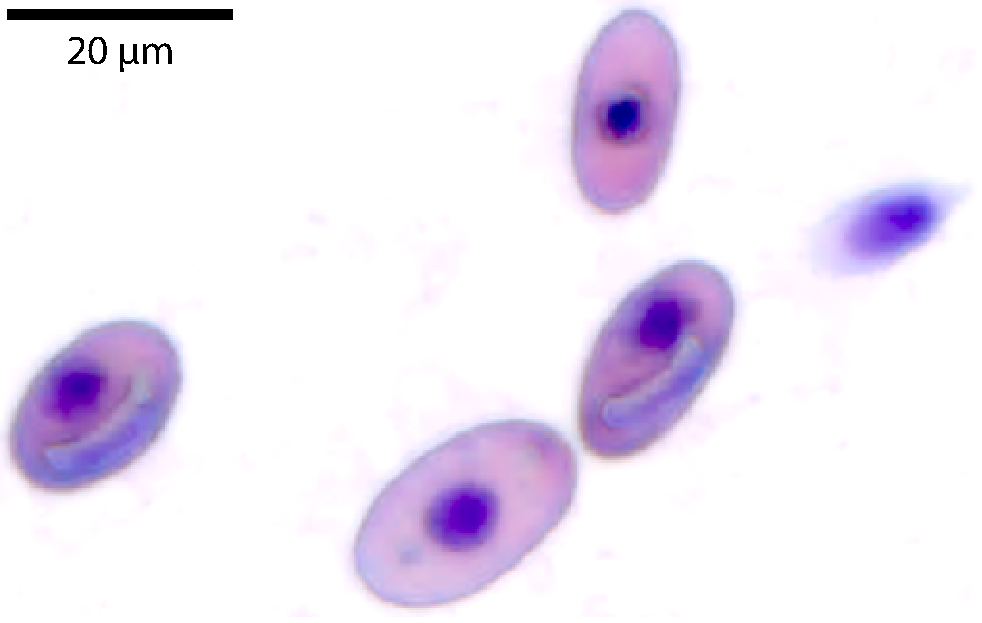
\includegraphics[width=16cm]{Figure_03.pdf}\par}
\vspace{0.3cm}{\legenda\RaggedRight \textbf{Figure 3.} Blood smear of \Bsaz{}. Two erythrocytes carry curved \Hep{} gamonts beside the host nucleus.\par}
\vfill
Only \textit{H.~atrocis} has shorter gamonts among the compared species (Fig.~4A). The gamont is short and broad (length/width 2.8), but its nucleus is long and narrow (length/width 2.1). No compared species combines the two (Fig.~4B).
\vfill
{\fontsize{30}{36}\selectfont\bfseries Two 18S variants that do not group together\par}\vspace{0.25cm}
The host carries two 18S rRNA variants (944 and 271 reads). Both fall inside \Hep{} (Fig.~5). V2 sits in a clade of Neotropical snake parasites (SH-aLRT 97.7, UFBoot 100), next to \textit{H.~annulatum}. V1 falls outside that clade, as sister to a group of snake and turtle parasites.
\end{minipage}\hfill
\usebox{\blocoquatro}
\end{minipage}}

% =====================================================================
%  COLUNA DIREITA
% =====================================================================
\newsavebox{\coldir}
\sbox{\coldir}{\begin{minipage}[t]{\coluna}\corpo\justifying\color{texto}
\vspace{-0.5cm}
\figura{44cm}{Figure_05.pdf}{\textbf{Figure 5.} Maximum likelihood tree of 150 adeleorin 18S rRNA sequences, rooted on \textit{Adelina}. Node labels: SH-aLRT/ultrafast bootstrap. Triangles: collapsed clades. Red: V1 and V2, the two variants from \Bsaz{}. Scale bar: substitutions per site.}

\subsecao{A large mitochondrial genome with a new gene order}
The mitochondrial genome is 10,479\,bp, 63\% longer than the largest published congener (6,413\,bp). It carries \textit{cox1}, \textit{cox3}, \textit{cob}, and 25 rRNA fragments, like its relatives. The extra length sits between \textit{cox1} and \textit{cob}, where \textit{cox3} now follows \textit{cob} (Fig.~7). The apicoplast genome is 32,316\,bp, with 22 protein-coding genes, 26 tRNA genes, and 4 rRNA genes (Fig.~6).
\figura{\linewidth}{Figure_06.pdf}{\textbf{Figure 6.} Apicoplast genome of \Hep{} sp. from \Bsaz{}, circular and drawn linear. Genes on the + strand sit above the line, genes on the \textminus{} strand below.}
\figura{\linewidth}{Figure_07.pdf}{\textbf{Figure 7.} Mitochondrial genomes of \Hep{}. Ribbons link \textit{cox1}, \textit{cox3}, and \textit{cob} between neighboring genomes.}

\secao{Conclusions}
\begin{itemize}
\item \Bsaz{} carries a \Hep{} lineage that differs from every compared species in gamont shape, 18S rRNA, and mitochondrial genome.
\item Its mitochondrial genome is the largest reported for the genus, with a gene order not seen before.
\item Two 18S variants in one host point to divergent rDNA copies or a mixed infection.
\item Host genome projects also sequence blood parasites, at no extra cost.
\end{itemize}
\end{minipage}}

\begin{document}
\typeout{ALTURA COLUNA ESQUERDA: \the\dimexpr\ht\colesq+\dp\colesq\relax}
\typeout{ALTURA COLUNA DIREITA: \the\dimexpr\ht\coldir+\dp\coldir\relax}
\begin{tikzpicture}[remember picture,overlay,x=1cm,y=1cm]
\color{texto}

% ================= CABECALHO =================
\node[anchor=north west,inner sep=0] at (\margem,-1.8cm) {%
\begin{minipage}[t]{66cm}\RaggedRight
{\fontsize{54}{62}\selectfont\bfseries\color{evento}
 Morphological and genomic characterization of a novel \Hep{} lineage in the critically endangered insular pitviper \Bsaz{} (Squamata: Serpentes: Viperidae)\par}
\vspace{0.8cm}
{\fontsize{34}{40}\selectfont
 \textbf{Pessoa, G.\,P.}\textsuperscript{1,4}, Salles-Oliveira, I.\textsuperscript{1,3}, Omura, G.\,Y.\,S.\textsuperscript{5}, Jacob Machado, D.\textsuperscript{5,6,*}, Nishiyama-Júnior, M.\,Y.\textsuperscript{2}, Silva, M.\,J.\,J.\textsuperscript{1,3}\par}
\vspace{0.5cm}
{\fontsize{22}{27}\selectfont
 \textsuperscript{1}Laboratório de Ecologia e Evolução, Instituto Butantan, São Paulo, Brazil.
 \textsuperscript{2}Laboratório de Toxinologia Aplicada, Instituto Butantan, São Paulo, Brazil.
 \textsuperscript{3}Instituto de Biociências, Universidade de São Paulo, São Paulo, Brazil.
 \textsuperscript{4}Instituto de Ciências Biomédicas, Universidade de São Paulo, São Paulo, Brazil.
 \textsuperscript{5}Department of Bioinformatics and Genomics, University of North Carolina at Charlotte, Charlotte, NC, USA.
 \textsuperscript{6}Center for Computational Intelligence for Predicting Health and Environmental Risks (CIPHER), University of North Carolina at Charlotte, Charlotte, NC, USA.
 \textsuperscript{*}dmachado@charlotte.edu\par}
\end{minipage}};

% logo do evento (obrigatorio) e logos das afiliacoes
\node[anchor=north east,inner sep=0] (logoevento) at (100cm-\margem,-1.8cm)
  {
\includegraphics[width=26cm]{Genetica.pdf}};
\node[anchor=north east,inner sep=0] (butantan) at ([yshift=-1.0cm]logoevento.south east)
  {
\includegraphics[height=\altlogo]{Butantan.pdf}};
\node[anchor=east,inner sep=0] (charlotte) at ([xshift=-1.2cm]butantan.west)
  {
\includegraphics[height=\altlogo]{Charlotte.png}};
\node[anchor=east,inner sep=0] (ib) at ([xshift=-1.2cm]charlotte.west)
  {
\includegraphics[height=\altlogo]{Bio.png}};

\fill[evento] (\margem,-15.0cm) rectangle (100cm-\margem,-15.3cm);

% ================= COLUNAS =================
\node[anchor=north west,inner sep=0] at (\margem,\topocolunas) {\usebox{\colesq}};
\node[anchor=north west,inner sep=0] at (\margem+\coluna+\vao,\topocolunas) {\usebox{\coldir}};

% ================= RODAPE =================
\fill[evento] (\margem,\toporodape+0.5cm) rectangle (100cm-\margem,\toporodape+0.35cm);
\node[anchor=north west,inner sep=0] at (\margem,\toporodape) {%
\begin{minipage}[t]{56cm}\rodape\RaggedRight\color{texto}
\textbf{Acknowledgments.} Instituto Butantan, Fundação Butantan, and Instituto de Biociências (USP) gave institutional support. The Núcleo de Bioinformática e Biologia Computacional (NBBC, Instituto Butantan) and the Department of Bioinformatics and Genomics (UNC Charlotte) gave computing infrastructure, and UNC Charlotte sequenced the samples. CAPES financed this study in part (Finance Code 001). We thank the Sociedade Brasileira de Genética for organizing Genética 2026. Animal use: CEUAIB protocol 8447060524. Genetic heritage access: SISGEN A4A6CA4.
\end{minipage}};
\node[anchor=north west,inner sep=0] at (\margem+57.5cm,\toporodape) {%
\begin{minipage}[t]{22cm}\rodape\RaggedRight\color{texto}
\textbf{References.} \textsuperscript{1}Barbo FE et al. 2016. Zootaxa 4097(4): 511-529. \textsuperscript{2}Barbo FE et al. 2022. Systematics and Biodiversity 20(1): 1-25.
\end{minipage}};
\node[anchor=north east,inner sep=0] (sbg) at (100cm-\margem,\toporodape+0.1cm)
  {
\includegraphics[height=\altlogorodape]{SBG.png}};
\node[anchor=north east,inner sep=0] at ([xshift=-1cm]sbg.north west)
  {
\includegraphics[height=\altlogorodape]{Capes.pdf}};

\end{tikzpicture}
\end{document}
